\subsection{Finding the Heart of the Folded Dipole!}
\begin{tcolorbox}[colback=gray!10, colframe=black, title=E9C07] What is the approximate feed point impedance at the center of a two-wire half-wave folded dipole antenna?
\begin{enumerate}[label=\Alph*.]
    \item \textbf{300 ohms}
    \item 72 ohms
    \item 50 ohms
    \item 450 ohms
\end{enumerate} \end{tcolorbox}

\subsubsection{Concepts Related to the Question}
The question pertains to the concept of feed point impedance in antennas, specifically the folded dipole antenna. A folded dipole antenna is a type of dipole that consists of two parallel wires. The configuration allows for an increase in the impedance due to the additional conductor.

\subsubsection{Understanding Feed Point Impedance}
In general, a standard half-wave dipole antenna has a feed point impedance of approximately 72 ohms when properly matched in free space. However, in the case of a folded dipole, the impedance is increased. The feed point impedance of a two-wire half-wave folded dipole is approximately four times that of a standard dipole due to the additional parallel path that the folded structure provides for the current.

To compute the feed point impedance \(Z_f\) of a folded dipole, we can use the following formula:
\[
Z_f = n^2 Z_{dipole}
\]
where \(n\) is the number of conductors in parallel and \(Z_{dipole}\) is the feed point impedance of a standard dipole.

For a folded dipole, we have:
- \(n = 2\) (since there are 2 parallel conductors)
- \(Z_{dipole} \approx 72 \text{ ohms}\)

Thus,
\[
Z_f = 2^2 \times 72 \text{ ohms} = 4 \times 72 \text{ ohms} = 288 \text{ ohms}
\]
This value is approximately categorized thus:
\[
Z_f \approx 300 \text{ ohms}
\]

\subsubsection{Conclusion}
Therefore, the correct choice from the given options is:
\textbf{A: 300 ohms}.

\subsubsection{Diagram}
To visualize a folded dipole antenna, we can utilize the TikZ package in LaTeX to draw a simple representation. Below is an illustrative diagram of a folded dipole antenna.

\begin{center}
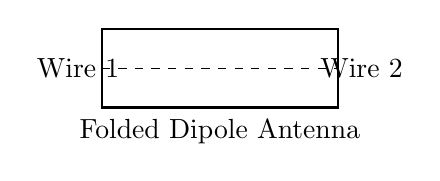
\begin{tikzpicture}
    \draw[thick] (0,0) -- (3,0) -- (3,1) -- (0,1) -- cycle; % Main wire
    \draw[thick] (0,0) -- (0,1); % Left vertical
    \draw[thick] (3,0) -- (3,1); % Right vertical
    \draw[dashed] (0,0.5) -- (3,0.5); % Midline
    \node at (1.5, -0.3) {Folded Dipole Antenna};
    \node at (-0.3, 0.5) {Wire 1};
    \node at (3.3, 0.5) {Wire 2};
\end{tikzpicture}
\end{center}
